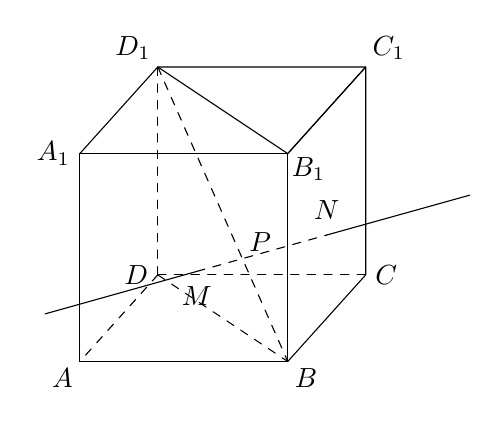
\begin{tikzpicture}[>=stealth, scale=1.1, line cap=round, line join=round]
  % Cube vertices
  \coordinate (A) at (0, 0);
  \coordinate (B) at (2.4, 0);
  \coordinate (B1) at (2.4, 2.4);
  \coordinate (A1) at (0, 2.4);

  \coordinate (D) at (0.9, 1.0);
  \coordinate (C) at (3.3, 1.0);
  \coordinate (C1) at (3.3, 3.4);
  \coordinate (D1) at (0.9, 3.4);

  % Dashed cube edges and diagonals
  \draw[dashed] (D) -- (D1);
  \draw[dashed] (D) -- (A);
  \draw[dashed] (D) -- (C);
  \draw[dashed] (D) -- (B);
  \draw[dashed] (D1) -- (B);

  % Point P on BD1
  \coordinate (P) at (1.875, 1.19);

  % Line MN
  \coordinate (Lstart) at (-0.4, 0.55);
  \coordinate (M) at (1.35, 1.04);
  \coordinate (N) at (2.85, 1.46);
  \coordinate (Lend) at (4.5, 1.92);

  \draw (Lstart) -- (M);
  \draw[dashed] (M) -- (N);
  \draw (N) -- (Lend);

  % Solid cube edges and diagonals
  \draw (A) -- (B) -- (B1) -- (A1) -- cycle;
  \draw (A1) -- (D1) -- (C1) -- (B1);
  \draw (B1) -- (C1) -- (C) -- (B);
  \draw (D1) -- (B1);

  % Labels
  \node[below left=-1pt] at (A) {$A$};
  \node[below right=-1pt] at (B) {$B$};
  \node[right] at (C) {$C$};
  \node[left] at (D) {$D$};
  \node[left] at (A1) {$A_1$};
  \node[below right=-2pt] at (B1) {$B_1$};
  \node[above right=-1pt] at (C1) {$C_1$};
  \node[above left=-1pt] at (D1) {$D_1$};

  \node[below=2pt] at (M) {$M$};
  \node[above=2pt] at (N) {$N$};
  \node[above right=-1pt] at (P) {$P$};
\end{tikzpicture}
